\documentclass[12pt]{article}
\usepackage{amsmath}
\usepackage{amssymb}
\usepackage{graphicx}
\usepackage{caption}
\usepackage[colorlinks=true, urlcolor=blue, linkcolor=red]{hyperref}
\usepackage{booktabs}
\usepackage{float}

% Setup
\captionsetup{font={small}}

\title{Fast Food Density Versus Median Income in Northwest Indiana Cities: A Bayesian Analysis}
\author{Adam Cuculich}
\date{December 2, 2023}

\begin{document}

\begin{titlepage}
\centering
\vspace*{\fill} % Add space above the title
\textbf{\Large Fast Food Density Versus Median Income\\
in Northwest Indiana Cities:\\[0.5em]
A Bayesian Analysis}\\[2em] % Title
\large ISyE 6420: Bayesian Statistics\\[0.5em] % Course title
\large Adam Cuculich\\[0.5em] % Author
\large December 2, 2023 % Date
\vspace*{\fill} % Add space below the center block
\end{titlepage}


\newpage

\section*{Introduction:}
\noindent This report presents an in-depth exploration of the potential relationship between the concentration of fast food restaurants, relative to dine-in, full-service establishments, and median household income in cities across Northwest Indiana. As someone who grew up in this region, I have some familiarity with the area, which inspired me to focus my research within this familiar context. Driven by a blend of curiosity and a desire for empirical understanding, this study aims to investigate whether a statistically significant relationship exists between these two variables, which, on the surface, might seem disconnected. A significant portion of this project was dedicated to the meticulous process of data acquisition and refinement. Recognizing the inherent limitations and uncertainties in the data, which was compiled from scratch, a Bayesian analytical approach was chosen for its robustness in handling uncertainty with limited data sets. Later in this report, I will discuss strategies for enhancing the dataset to improve the reliability and depth of future studies. In the interest of open-source analysis, all relevant code files are available on \href{https://github.com/cucupac/bayesian-stats/tree/main/project}{GiHub}. The goal is to provide a foundation that not only reveals insights about the current data but also paves the way for more comprehensive research in this area.

\section*{Methodology}

The methodology of this investigation is structured methodically to examine the relationship between fast food restaurant density and median household income in Northwest Indiana. The study focuses on cities and towns within Lake and Porter Counties with populations exceeding 500. The investigative process involves several key steps:

\paragraph{Identification of Cities}
The first step is to compile a comprehensive list of cities in Northwest Indiana, defined by their geographical location within Lake or Porter County and having a population above the specified threshold.

\paragraph{Geographical Centering}
For each city, the central point is determined based on its latitudinal and longitudinal coordinates. This geographical center serves as the focal point for subsequent data collection.

\paragraph{Restaurant Data Collection}
Utilizing the city center coordinates, the next step involves gathering data on restaurants within a 5-kilometer radius of each center. This data collection provides a basis upon which restaurants can be later categorized.

\paragraph{Restaurant Categorization}
Restaurants are classified into two distinct categories: fast food and full-service dine-in establishments. The classification criteria are based on common understanding and operational definitions for this study. Fast food restaurants are identified as those generally recognized as such or primarily offering takeaway services. In contrast, the remaining restaurants are categorized as full-service, where customers dine in and receive table service.

\paragraph{Income Data Collection}
Median household income data for each city was gathered as a critical socio-economic variable. This data, combined with the restaurant information, allows for the analysis of potential correlations between fast food restaurant density and economic indicators in the studied cities.

\paragraph{Analysis Preparation}
Following data collection, the next phase focused on preparing for the analysis. This involved calculating the proportion of fast food establishments relative to the total number of restaurants in each city, thus quantifying the density of fast food options. The study then set out to explore the potential correlation between two primary variables: the density of fast food restaurants and the median household income.

\paragraph{Bayesian Linear Regression Model}
To analyze the data, a Bayesian linear regression model is employed using probabilistic programming. This approach allows for a nuanced analysis, taking into account the uncertainties and variabilities inherent in the data. The model aims to determine whether or not there is a significant correlation between the density of fast food restaurants and the median household income in the studied areas. \\

\noindent Throughout this process, the methodology was applied with a commitment to thoroughness within the time and resource constraints of the study. While acknowledging the challenges in accurately classifying restaurant types and handling geographical and demographic data, strong efforts were made to ensure the reliability of the analysis.

\section*{Data Acquisition}

\paragraph{Identification of Cities}
The compilation of the list of cities in Lake and Porter Counties was sourced from \href{https://geographic.org/streetview/usa/in/lake/index.html}{geographic.org}. The website provides an interface where specifying a county name yields a comprehensive list of cities within that county. The list of cities was then refined to only include cities or towns with a population greater than 500. Population numbers were obtained form \texttt{api.census.gov}, using FIPS codes for each city. The code that implements this work can be found in the attached \href{https://github.com/cucupac/bayesian-stats/blob/main/project/data_collection/get_population_data.py}{\texttt{get\_population\_data.py}} file.

\paragraph{Geographical Centering}
To determine the geographical centers of these cities, the Python library Geopy was employed. By inputting a city name and using the \texttt{indiana\_geocoder} user agent, Geopy returns the latitude and longitude coordinates for each city. The implementation details and code are available in the attached \href{https://github.com/cucupac/bayesian-stats/blob/main/project/data_collection/get_coordinates.py}{\texttt{get\_coordinates.py}} file.


\paragraph{Restaurant Data Collection}
Utilizing the GPS coordinates obtained from the Geopy library, the Google Places API was instrumental in gathering lists of restaurants within a 5-kilometer radius of each city's coordinates. The data for each city was recorded in separate CSV files. All retrieved data is stored in the \href{https://github.com/cucupac/bayesian-stats/tree/main/project/restaurants}{\texttt{restaurants directory}}, and the code for this task is outlined in the \href{https://github.com/cucupac/bayesian-stats/blob/main/project/data_collection/get_restaurant_data.py}{\texttt{get\_restaurant\_data.py}} file.

\paragraph{Restaurant Categorization}
Categorizing the restaurants posed a significant challenge. Initially, the \texttt{meal\_takeaway} tag from the Google Places API's returned objects was considered as a categorization criterion. However, this method was found to be unreliable, as many obvious fast food establishments lacked this tag. Consequently, the lists of restaurants were provided to ChatGPT4 for classification into two categories: fast-food, takeout restaurants and full-service, dine-in establishments. While this method may not conform to a strict mathematical categorization technique, it produced reasonable results for the purposes of this analysis. The resulting list of fast food establishments used for the study can be found in the \href{https://github.com/cucupac/bayesian-stats/blob/main/project/data_collection/fastfood.py}{\texttt{fastfood.py}} file, stored as a variable named, \texttt{FAST\_FOOD\_LIST}. Further discussion on improving this methodology is included later in the report.

\paragraph{Income Data Collection}
The acquisition of median household income data commenced with obtaining FIPS codes corresponding to each city's GPS coordinates, facilitated by \texttt{api.census.gov}, as detailed in the \href{https://github.com/cucupac/bayesian-stats/blob/main/project/data_collection/get_fips_code.py}{\texttt{get\_fips\_codes.py}} file. Subsequently, these FIPS codes were used to retrieve the median household income data for each city, with the implementation detailed in the \href{https://github.com/cucupac/bayesian-stats/blob/main/project/data_collection/get_income_data.py}{\texttt{get\_income\_data.py}} file.

\paragraph{Analysis Preparation}
Following the comprehensive data collection process, the fast food density for each city was computed using the script provided in the \href{https://github.com/cucupac/bayesian-stats/blob/main/project/data_collection/get_fastfood_percentage.py}{\texttt{get\_fastfood\_percentage.py}} file. The culmination of the collected data, which forms the basis for our subsequent Bayesian analysis, is succinctly summarized in the table below:

% Image
\begin{figure}[h!]
\centering
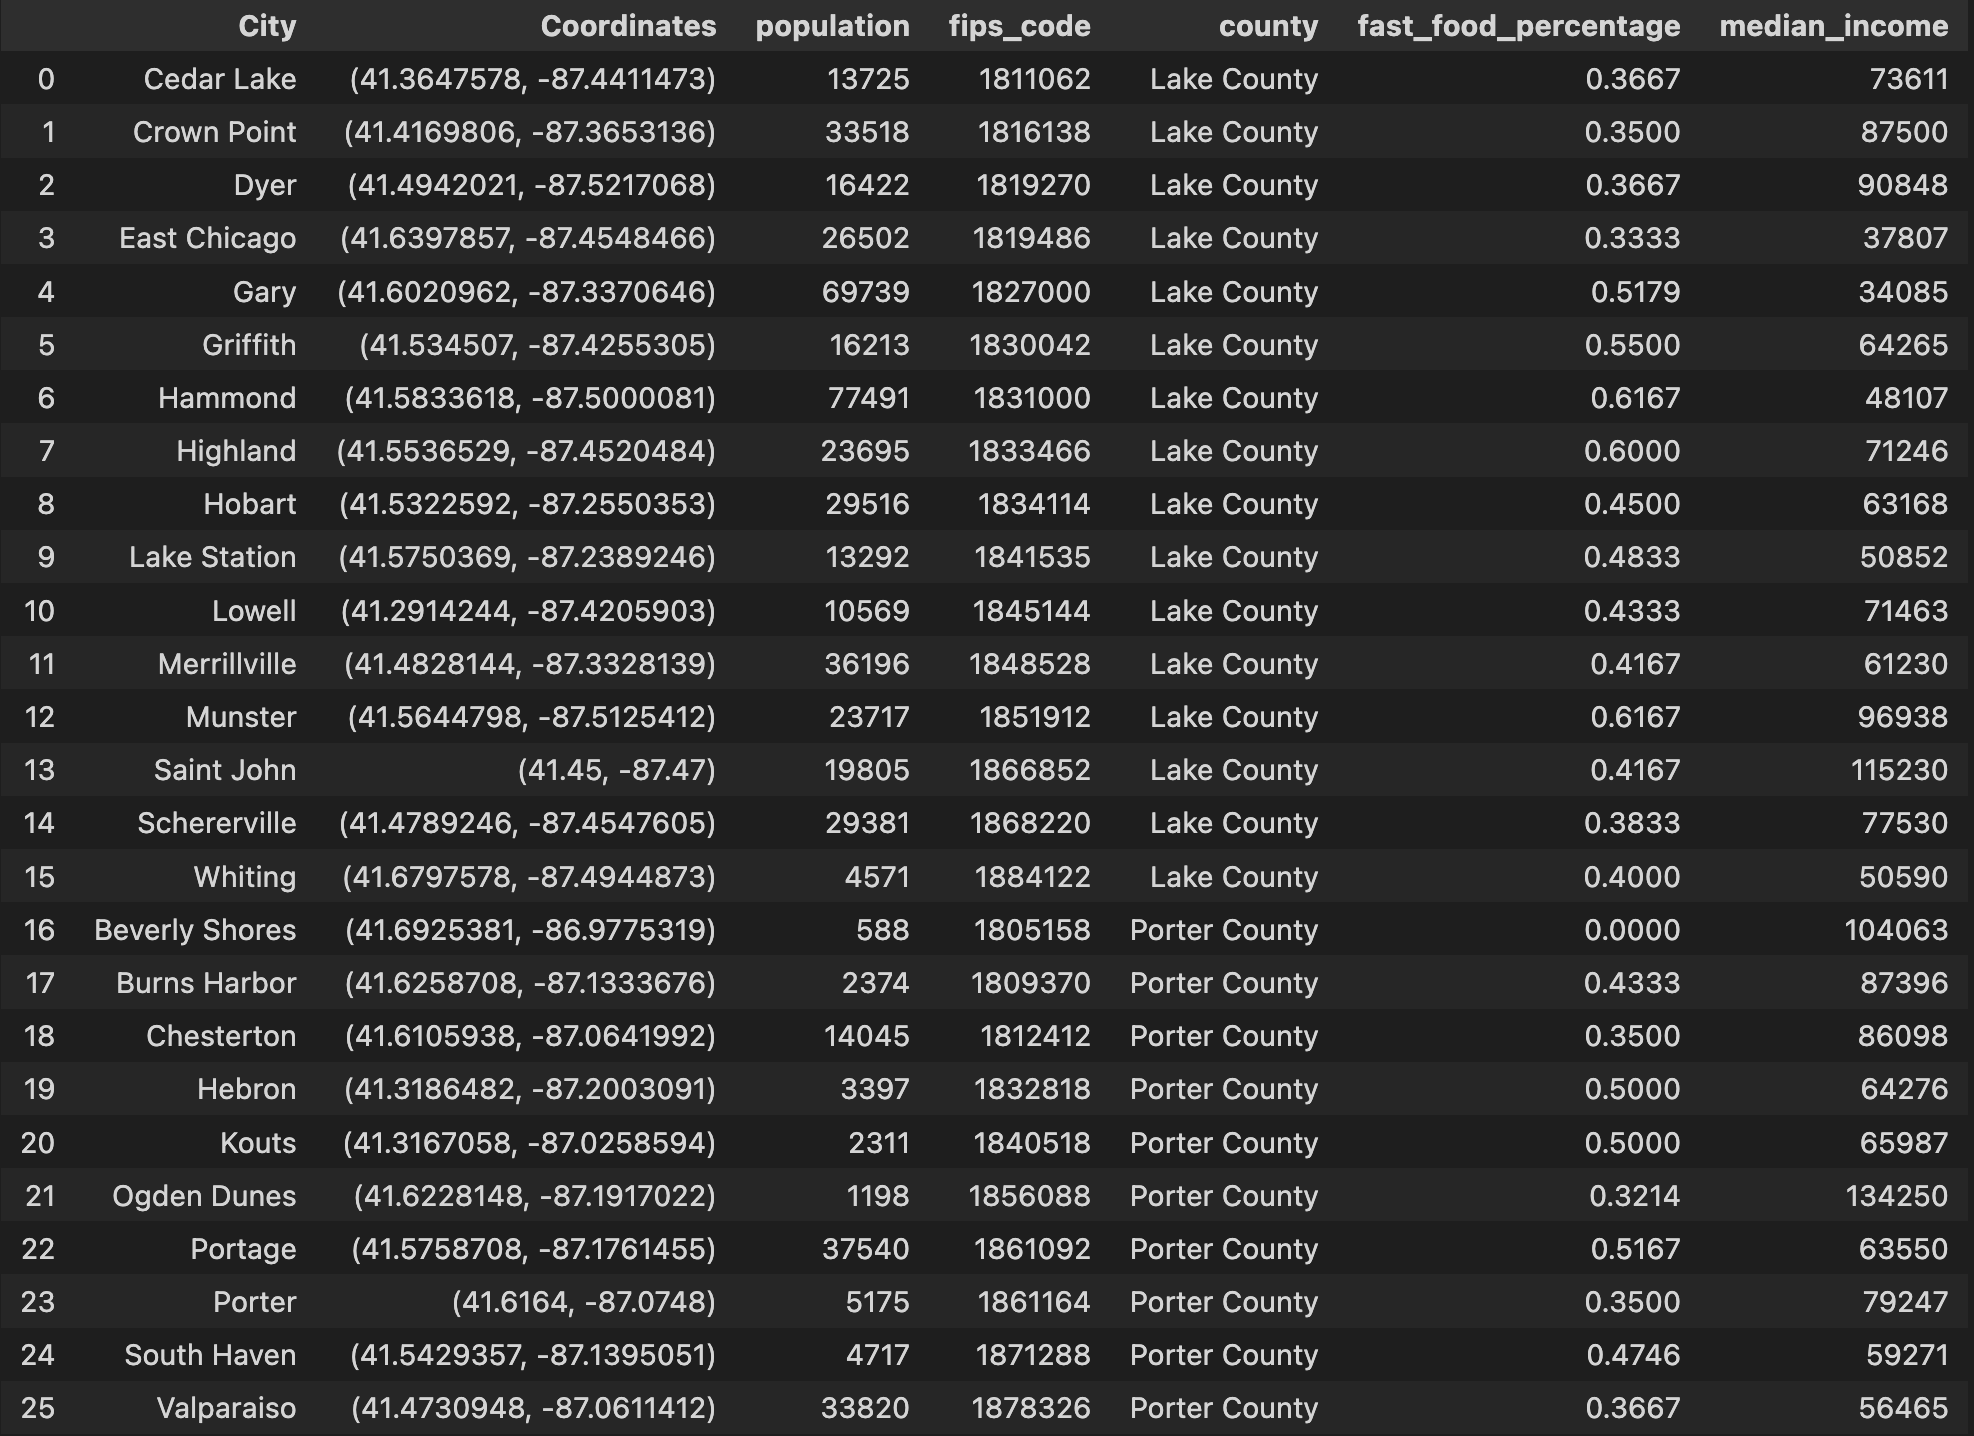
\includegraphics[width=1.0\textwidth]{../assets/data_table.png} 
\caption{Data obtained for Bayesian analysis}
\label{fig:cond_prob}
\end{figure}

\paragraph{Bayesian Linear Regression Model}
The relationship between fast food density and median income was analyzed using a Bayesian Linear Regression model in PyMC3. Key components of the model included standardized data input, specified priors (Normal for intercept and beta, Gamma for precision), a linear function relating median income to fast food percentage, and a likelihood function. The model was calibrated with 3000 posterior samples to ensure robustness. This approach allowed for an in-depth, probabilistic understanding of the relationship between the two variables. The detailed implementation is available in the \href{https://github.com/cucupac/bayesian-stats/blob/main/project/bayesian_analysis_ffp.ipynb}{\texttt{bayesian\_anaylsis\_ffp.ipynb}} file. The code below illustrates the core components of the model, were \texttt{ffp} and \texttt{mi} stand for "fast food percentage" and "median income", respectively:

% Image
\begin{figure}[h!]
\centering
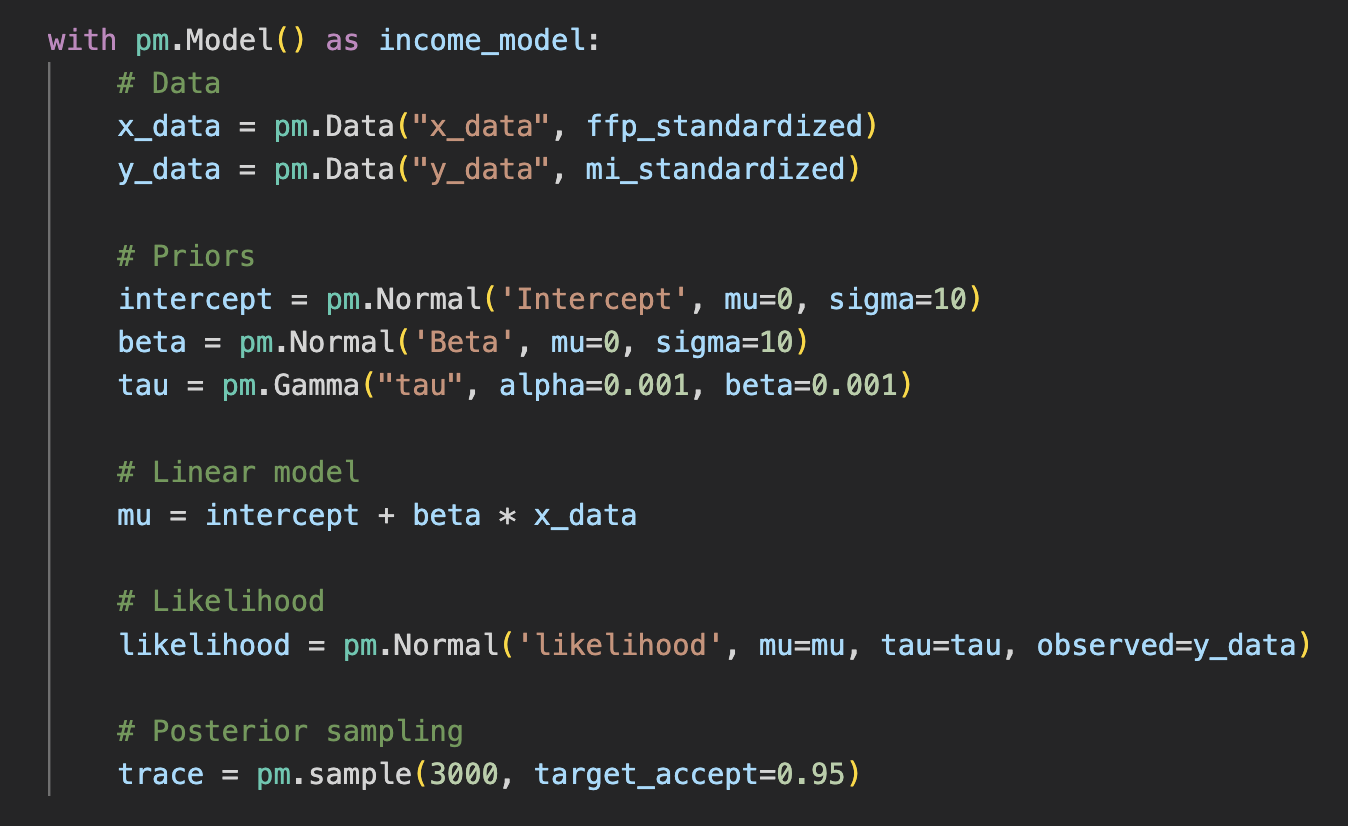
\includegraphics[width=1.0\textwidth]{../assets/model.png} 
\caption{A Bayesian linear regression model}
\label{fig:cond_prob}
\end{figure}

\newpage
\section*{Results}

\noindent The Bayesian analysis conducted on the data resulted in a posterior distribution for the model parameters, which provides insights into the relationship between fast food restaurant density and median household income. The summary statistics of the posterior distributions for each parameter are presented in the following table:

% Image
\begin{figure}[h!]
\centering
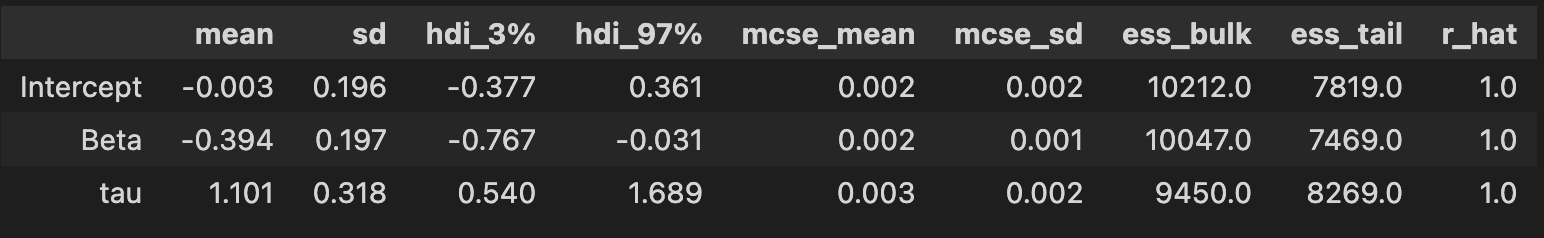
\includegraphics[width=1.0\textwidth]{../assets/results.png} 
\caption{Posterior Summary Statistics}
\label{fig:cond_prob}
\end{figure}

\noindent The HDI for the beta parameter, ranging from -0.767 to -0.031, lies entirely below zero, suggesting with 94\% confidence that an increase in fast-food restaurant density correlates with a decrease in median household income. This negative association, while statistically significant, comes with a caveat — the broad range of the HDI indicates considerable uncertainty about the magnitude of this effect. The scatter of data points around the following regression line further suggests that the predictive power of fast-food density on median income, while present, may not be strong.

% Image
\begin{figure}[h!]
\centering
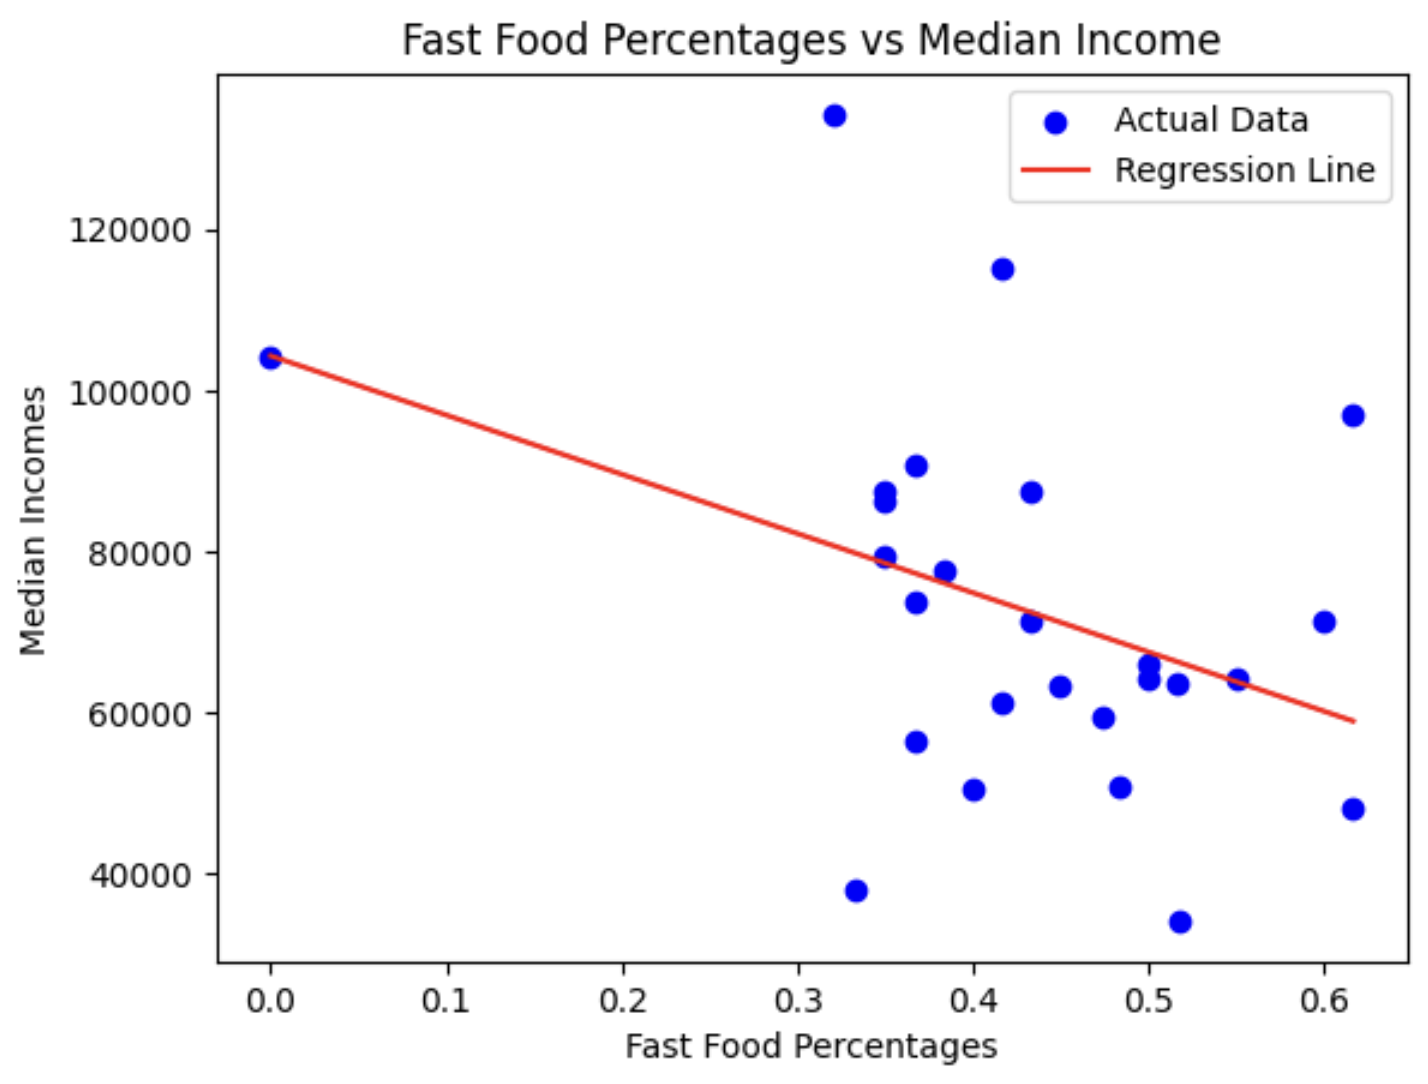
\includegraphics[width=0.9\textwidth]{../assets/regression.png} 
\caption{Fast food density compared to median household income}
\label{fig:cond_prob}
\end{figure}

\newpage
\section*{Suggested Improvements}

\paragraph{Restaurant Data}
The current analysis is limited by a Google Places API's restriction, which yields a maximum of 60 restaurants for a given area. This constraint almost certainly results in an incomplete dataset, potentially affecting the robustness of the study. To mitigate this limitation, incorporating additional data sources, such as the Yelp API, could enhance the comprehensiveness of restaurant discovery and provide a more accurate representation of the fast-food landscape.

\paragraph{Restaurant Categorization}
The method of categorizing restaurants employed in this study relies on ChatGPT4's classification, which, while efficient, lacks systematic rigor. Future research could benefit from a more structured approach, possibly by leveraging multiple tags from both Google and Yelp data sources to classify restaurants more precisely. Furthermore, incorporating metrics such as the average duration of restaurant visits, if accessible, could serve as a more objective measure to differentiate between fast-food and full-service, sit-down restaurants. Such data could refine the categorization process, leading to potentially more insightful results.

\section*{Conclusion:}
\noindent Through Bayesian analysis, this study has identified a negative correlation between fast-food restaurant density and median household income within Northwest Indiana. Given the data collection limitations and the significant variance observed in the data points, the results suggest a cautious interpretation. The extensive HDIs underscore the necessity of further, more rigorous research before making definitive assertions about the relationship identified. Recommendations for future research include expanding the dataset beyond the Google Places API's restrictions and enhancing restaurant categorization methods. The study provides a preliminary understanding of the economic factors associated with fast-food restaurant distribution and emphasizes the need for a more detailed investigation to ascertain these findings with greater confidence. The analysis, while not conclusive on its own, sets the stage for subsequent inquiries into these complex socio-economic interactions.


\end{document}
